% gen_statem Usage Guide
% A complete introduction to gen_statem with architecture diagrams and examples.
% Compile with: xelatex gen_statem_architecture.tex (run twice for TOC)
\documentclass[a4paper,11pt]{article}

% ============================================================
% Packages
% ============================================================
\usepackage{fontspec}
\usepackage{xeCJK}
\setCJKmainfont[BoldFont=STHeiti, ItalicFont=STKaiti]{STSong}
\setCJKsansfont{STHeiti}
\setCJKmonofont{STFangsong}

\usepackage[margin=2.5cm]{geometry}
\usepackage{graphicx}
\usepackage{xcolor}
\usepackage{hyperref}
\usepackage{listings}
\usepackage{booktabs}
\usepackage{longtable}
\usepackage{enumitem}
\usepackage{tikz}
\usepackage{tcolorbox}
\usepackage{fancyhdr}
\usepackage{titlesec}
\usepackage{amsmath}
\usepackage{amssymb}
\usepackage{float}
\usepackage{pifont}

\usetikzlibrary{arrows.meta, positioning, shapes.geometric, fit, calc, backgrounds, decorations.pathreplacing}

\tcbuselibrary{listings, skins, breakable}

% ============================================================
% Color Definitions
% ============================================================
\definecolor{erlred}{HTML}{A4070A}
\definecolor{erlblue}{HTML}{2B5EA7}
\definecolor{erlgreen}{HTML}{2E7D32}
\definecolor{erlyellow}{HTML}{F9A825}
\definecolor{erlpurple}{HTML}{6A1B9A}
\definecolor{erlmodule}{HTML}{D84315}
\definecolor{erlinit}{HTML}{00897B}
\definecolor{erlpid}{HTML}{E65100}
\definecolor{erlname}{HTML}{6A1B9A}
\definecolor{codebg}{HTML}{F5F5F5}
\definecolor{codeborder}{HTML}{CCCCCC}
\definecolor{tipbg}{HTML}{E8F5E9}
\definecolor{warnbg}{HTML}{FFF3E0}
\definecolor{notebg}{HTML}{E3F2FD}
\definecolor{darkgray}{HTML}{333333}

% ============================================================
% Hyperref Setup
% ============================================================
\hypersetup{
    colorlinks=true,
    linkcolor=erlblue,
    urlcolor=erlpurple,
    citecolor=erlgreen,
    pdftitle={gen\_statem 用法指南},
    pdfauthor={Erlang OTP Tutorial},
    bookmarksnumbered=true,
}

% ============================================================
% Code Listing Style
% ============================================================
\lstdefinelanguage{erlang}{
    morekeywords={module, export, import, behaviour, behavior, spec, type,
        record, define, include, ifdef, ifndef, else, endif, undef,
        case, of, end, if, receive, after, when, fun, try, catch, throw,
        begin, spawn, spawn_link, register, self, send, ok, error,
        true, false, undefined, infinity, timeout, noreply, reply, stop,
        hibernate, ignore, normal, process_flag, trap_exit, monitor_node},
    sensitive=true,
    morecomment=[l]{\%},
    morestring=[b]",
    morestring=[b]',
}

\lstdefinestyle{erlangstyle}{
    language=erlang,
    basicstyle=\ttfamily\small,
    keywordstyle=\color{erlblue}\bfseries,
    commentstyle=\color{erlgreen}\itshape,
    stringstyle=\color{erlred},
    numberstyle=\tiny\color{gray},
    numbers=left,
    numbersep=8pt,
    backgroundcolor=\color{codebg},
    frame=single,
    rulecolor=\color{codeborder},
    breaklines=true,
    breakatwhitespace=true,
    tabsize=4,
    showstringspaces=false,
    captionpos=b,
    xleftmargin=1.5em,
    framexleftmargin=1em,
    aboveskip=1em,
    belowskip=0.8em,
}

\lstdefinestyle{shellstyle}{
    basicstyle=\ttfamily\small\color{white},
    backgroundcolor=\color{darkgray},
    rulecolor=\color{darkgray},
    frame=single,
    breaklines=true,
    showstringspaces=false,
    xleftmargin=1.5em,
    framexleftmargin=1em,
    aboveskip=1em,
    belowskip=0.8em,
}

\lstset{style=erlangstyle}

% ============================================================
% Custom tcolorbox Environments
% ============================================================
\newtcolorbox{tipbox}[1][]{
    colback=tipbg, colframe=erlgreen!80!black,
    fonttitle=\bfseries, title={#1},
    arc=2mm, boxrule=0.8pt,
    left=6pt, right=6pt, top=4pt, bottom=4pt,
    breakable,
}

\newtcolorbox{warnbox}[1][]{
    colback=warnbg, colframe=erlyellow!80!black,
    fonttitle=\bfseries, title={#1},
    arc=2mm, boxrule=0.8pt,
    left=6pt, right=6pt, top=4pt, bottom=4pt,
    breakable,
}

\newtcolorbox{notebox}[1][]{
    colback=notebg, colframe=erlblue!80!black,
    fonttitle=\bfseries, title={#1},
    arc=2mm, boxrule=0.8pt,
    left=6pt, right=6pt, top=4pt, bottom=4pt,
    breakable,
}

% ============================================================
% Header / Footer
% ============================================================
\pagestyle{fancy}
\fancyhf{}
\fancyhead[L]{\small\textit{gen\_statem 用法指南}}
\fancyhead[R]{\small\textit{Erlang/OTP}}
\fancyfoot[C]{\thepage}
\renewcommand{\headrulewidth}{0.4pt}

% ============================================================
% Title Formatting
% ============================================================
\titleformat{\section}
    {\LARGE\bfseries\color{erlblue}}
    {\thesection}{1em}{}[\vspace{-0.5em}\rule{\textwidth}{0.8pt}]

\titleformat{\subsection}
    {\Large\bfseries\color{erlblue!80!black}}
    {\thesubsection}{0.8em}{}

\titleformat{\subsubsection}
    {\large\bfseries\color{erlblue!60!black}}
    {\thesubsubsection}{0.6em}{}

% ============================================================
% Document Begin
% ============================================================
\begin{document}

% ---- Title Page ----
\begin{titlepage}
\centering
\vspace*{3cm}

{\fontsize{42}{48}\selectfont\bfseries\color{erlblue} gen\_statem}\\[12pt]
{\fontsize{24}{28}\selectfont\color{erlblue!70!black} 用法指南}

\vspace{2cm}

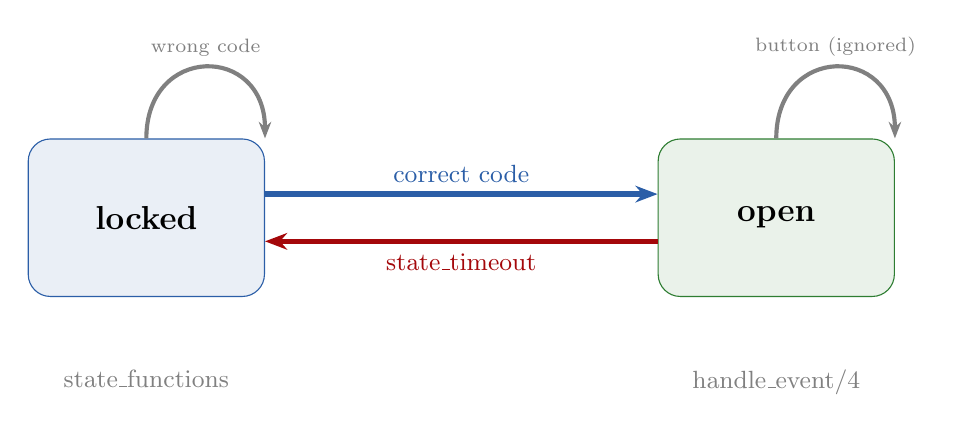
\begin{tikzpicture}
    % States
    \node[draw=erlblue, fill=erlblue!10, rounded corners=8pt, minimum width=3cm, minimum height=2cm, font=\large\bfseries] (locked) at (0,0) {locked};
    \node[draw=erlgreen, fill=erlgreen!10, rounded corners=8pt, minimum width=3cm, minimum height=2cm, font=\large\bfseries] (open) at (8,0) {open};

    % Transitions
    \draw[-{Stealth[length=8pt]}, line width=2pt, erlblue]
        ([yshift=3mm]locked.east) -- node[above, font=\small] {correct code} ([yshift=3mm]open.west);
    \draw[-{Stealth[length=8pt]}, line width=2pt, erlred]
        ([yshift=-3mm]open.west) -- node[below, font=\small] {state\_timeout} ([yshift=-3mm]locked.east);

    % Self-loops
    \draw[-{Stealth[length=6pt]}, line width=1.5pt, gray]
        (locked.north) .. controls ++(0,1.2) and ++(0,1.2) .. node[above, font=\scriptsize] {wrong code} (locked.north east);
    \draw[-{Stealth[length=6pt]}, line width=1.5pt, gray]
        (open.north) .. controls ++(0,1.2) and ++(0,1.2) .. node[above, font=\scriptsize] {button (ignored)} (open.north east);

    \node[below=8mm of locked, font=\small\color{gray}] {state\_functions};
    \node[below=8mm of open, font=\small\color{gray}] {handle\_event/4};
\end{tikzpicture}

\vspace{3cm}

{\large\color{darkgray} 以 code\_lock 为例，从架构到实践}

\vspace{1cm}

{\normalsize\color{gray} Erlang/OTP $\cdot$ Behavior Pattern $\cdot$ State Machine Programming}

\vfill
{\small\today}
\end{titlepage}

% ---- Table of Contents ----
\newpage
\tableofcontents
\newpage


% ============================================================
% Section 1: Overview
% ============================================================
\section{概述}

\subsection{什么是 gen\_statem？}

\texttt{gen\_statem} 是 OTP 框架中的\textbf{通用状态机}行为模式（behavior），是 \texttt{gen\_fsm} 的替代品（OTP 20+）。它提供了两种回调模式，支持丰富的状态转换动作，是实现有限状态机的首选方案。

\begin{tipbox}[核心思想]
\textbf{gen\_statem = State Machine Engine + Callback Module}

\begin{itemize}[leftmargin=1.5em]
    \item \textbf{State Machine Engine}（\texttt{gen\_statem.erl}）：消息循环、状态路由、超时管理、事件队列
    \item \textbf{Callback Module}（你的回调模块）：定义状态、处理事件、执行状态转换
    \item 两种回调模式：\texttt{state\_functions}（每个状态一个函数）和 \texttt{handle\_event\_function}（统一处理函数）
\end{itemize}
\end{tipbox}

\subsection{核心概念}

\begin{figure}[H]
\centering
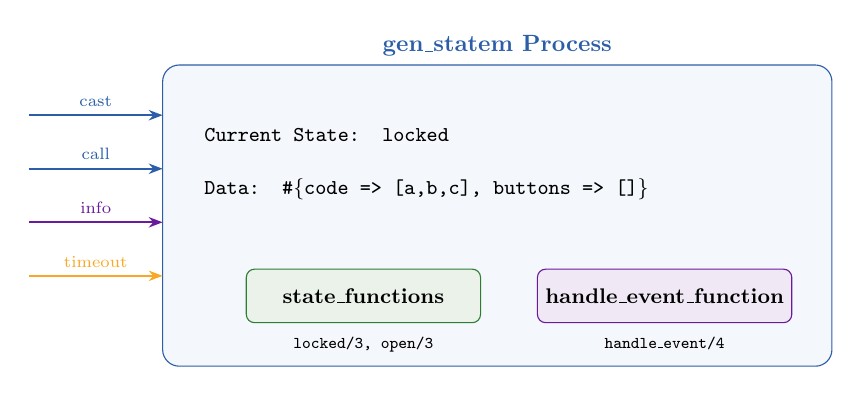
\begin{tikzpicture}[scale=0.85, every node/.style={scale=0.85}]
    \node[draw=erlblue, fill=erlblue!5, rounded corners=6pt, minimum width=10cm, minimum height=4.5cm] (proc) at (0,0) {};
    \node[above=0pt of proc.north, font=\bfseries\color{erlblue}] {gen\_statem Process};

    \node[font=\small\ttfamily, anchor=west] at (-4.5, 1.2) {Current State: \textbf{locked}};
    \node[font=\small\ttfamily, anchor=west] at (-4.5, 0.4) {Data: \#\{code => [a,b,c], buttons => []\}};

    \node[draw=erlgreen, fill=erlgreen!10, rounded corners=3pt, minimum width=3.5cm, minimum height=0.8cm, font=\small\bfseries] (sf) at (-2, -1.2) {state\_functions};
    \node[draw=erlpurple, fill=erlpurple!10, rounded corners=3pt, minimum width=3.5cm, minimum height=0.8cm, font=\small\bfseries] (hef) at (2.5, -1.2) {handle\_event\_function};

    \node[font=\scriptsize\ttfamily, below=2pt of sf] {locked/3, open/3};
    \node[font=\scriptsize\ttfamily, below=2pt of hef] {handle\_event/4};

    % Incoming events
    \draw[-{Stealth[length=5pt]}, thick, erlblue] (-7, 1.5) -- node[above, font=\scriptsize] {cast} (-5, 1.5);
    \draw[-{Stealth[length=5pt]}, thick, erlblue] (-7, 0.7) -- node[above, font=\scriptsize] {call} (-5, 0.7);
    \draw[-{Stealth[length=5pt]}, thick, erlpurple] (-7, -0.1) -- node[above, font=\scriptsize] {info} (-5, -0.1);
    \draw[-{Stealth[length=5pt]}, thick, erlyellow] (-7, -0.9) -- node[above, font=\scriptsize] {timeout} (-5, -0.9);
\end{tikzpicture}
\caption{gen\_statem 进程内部结构}
\end{figure}

\subsection{gen\_statem 提供的能力}

\begin{table}[H]
\centering
\begin{tabular}{@{}ll@{}}
\toprule
\textbf{能力} & \textbf{说明} \\
\midrule
两种回调模式         & \texttt{state\_functions} 和 \texttt{handle\_event\_function} \\
同步调用 (call)      & 客户端发送请求并等待回复 \\
异步调用 (cast)      & 客户端发送请求后立即返回 \\
Event Timeout        & 任何事件到达都会取消 \\
State Timeout        & 状态变化时自动取消 \\
Generic Timeout      & 命名超时，只能显式取消 \\
State Enter          & 每次状态变化时执行进入动作 \\
Postpone             & 将事件推迟到状态变化后重新处理 \\
Next Event           & 在当前状态插入新事件 \\
复杂状态             & 状态可以是任意 term，不限于 atom \\
热代码升级           & 通过 \texttt{code\_change/4} 支持运行时升级 \\
\bottomrule
\end{tabular}
\caption{gen\_statem 提供的能力}
\end{table}

\subsection{OTP 源码中的工作流}

以下直接对应 \texttt{gen\_statem.erl} 源码中的注释：

\begin{tcolorbox}[colback=codebg, colframe=codeborder, arc=2mm, boxrule=0.5pt,
                  title={\textbf{gen\_statem.erl --- Work Flow (state\_functions)}},
                  fonttitle=\bfseries\ttfamily, width=\textwidth]
\small\ttfamily
\begin{tabular}{@{}lcl@{}}
gen\_statem module &  & Callback module \\
\textsf{-{}-{}-{}-{}-{}-{}-{}-{}-{}-{}-{}-{}-{}-{}-{}-{}-} & & \textsf{-{}-{}-{}-{}-{}-{}-{}-{}-{}-{}-{}-{}-{}-{}-} \\
gen\_statem:start\_link & -{}-{}-{}-{}-> & Module:init/1 \\
gen\_statem:cast        & -{}-{}-{}-{}-> & Module:StateName/3 \\
gen\_statem:call        & -{}-{}-{}-{}-> & Module:StateName/3 \\
-                      & -{}-{}-{}-{}-> & Module:StateName/3 (info) \\
-                      & -{}-{}-{}-{}-> & Module:StateName/3 (timeout) \\
-                      & -{}-{}-{}-{}-> & Module:StateName/3 (enter) \\
gen\_statem:stop        & -{}-{}-{}-{}-> & Module:terminate/3 \\
-                      & -{}-{}-{}-{}-> & Module:code\_change/4 \\
\end{tabular}
\end{tcolorbox}

\subsection{与 gen\_server / gen\_fsm 的对比}

\begin{table}[H]
\centering
\begin{tabular}{@{}llll@{}}
\toprule
\textbf{特性} & \textbf{gen\_server} & \textbf{gen\_fsm} & \textbf{gen\_statem} \\
\midrule
状态概念     & 隐式（在 State 中） & 显式（atom 状态名） & 显式（任意 term） \\
回调模式     & 单一               & state\_functions   & state\_functions / handle\_event \\
超时类型     & timeout            & timeout            & event / state / generic \\
state\_enter & \ding{55}          & \ding{55}          & \ding{51} \\
postpone     & \ding{55}          & \ding{55}          & \ding{51} \\
next\_event  & \ding{55}          & \ding{55}          & \ding{51} \\
复杂状态     & N/A                & \ding{55} (atom)   & \ding{51} (any term) \\
OTP 版本     & 始终可用           & 已废弃             & OTP 19+ \\
\bottomrule
\end{tabular}
\caption{gen\_server vs gen\_fsm vs gen\_statem}
\end{table}


% ============================================================
% Section 2: Architecture Diagrams (PID)
% ============================================================
\section{架构图（通过 Pid）}

使用 \texttt{gen\_statem:start\_link(Module, Args, Opts)} 启动，不注册名字，通过返回的 Pid 来引用状态机。

\begin{figure}[H]
\centering
\includegraphics[width=\textwidth]{images/gen_statem_architecture_pid.pdf}
\caption{架构图（方式一）：通过 PID 引用 --- \texttt{start\_link/3}}
\label{fig:arch-pid}
\end{figure}

\subsection{不注册（使用 PID）}

\begin{lstlisting}[style=erlangstyle]
{ok, Pid} = gen_statem:start_link(?MODULE, Code, []).
%% Call by PID:
gen_statem:call(Pid, Request).
%% Cast by PID:
gen_statem:cast(Pid, {button, a}).
%% Stop by PID:
gen_statem:stop(Pid).
\end{lstlisting}

\subsection{实验演示：本地 PID 场景}

在同一个 Erlang 节点上启动匿名 gen\_statem，通过返回的 PID 直接操作。

\begin{lstlisting}[style=shellstyle, caption={PID 场景 --- 匿名 gen\_statem}]
(apple@ERICKSUN-MC1)1> {ok, Pid} = lock_state_pid:start_link(
    [a, b, c]).
Lock
{ok,<0.93.0>}
(apple@ERICKSUN-MC1)2> lock_state_pid:button(Pid, a).
ok
(apple@ERICKSUN-MC1)3> lock_state_pid:button(Pid, b).
ok
(apple@ERICKSUN-MC1)4> lock_state_pid:button(Pid, c).
Unlock
ok
(apple@ERICKSUN-MC1)5> lock_state_pid:stop(Pid).
ok
\end{lstlisting}

\begin{notebox}[PID 方式的特点]
\begin{itemize}[leftmargin=1.5em]
    \item PID 是进程的直接引用，无需名字注册
    \item 可以启动多个匿名 gen\_statem 实例
    \item PID 仅在本地节点有效，跨节点需要额外处理
    \item 必须自行保存 PID，进程死亡后 PID 失效
\end{itemize}
\end{notebox}


% ============================================================
% Section 3: Architecture Diagrams (Named)
% ============================================================
\section{架构图（通过名字）}

使用 \texttt{gen\_statem:start\_link(ServerName, Module, Args, Opts)} 启动，将状态机注册到名字表，通过名字引用。

\begin{figure}[H]
\centering
\includegraphics[width=\textwidth]{images/gen_statem_architecture_named.pdf}
\caption{架构图（方式二）：通过注册名字引用 --- \texttt{start\_link/4}}
\label{fig:arch-named}
\end{figure}

gen\_statem 支持多种进程注册方式：

\subsection{本地注册}

\begin{lstlisting}[style=erlangstyle]
gen_statem:start_link({local, code_lock}, ?MODULE, Code, []).
%% All operations use the atom name:
gen_statem:cast(code_lock, {button, a}).
gen_statem:call(code_lock, get_status).
gen_statem:stop(code_lock).
%% Only visible on current node
\end{lstlisting}

\paragraph{实验演示：本地注册在集群中互不影响}

本地注册（\texttt{\{local, Name\}}）的名字仅在当前节点可见。在集群中，\textbf{每个节点可以各自注册同名状态机，互不影响}。

\textbf{节点 apple} --- 启动并注册 \texttt{lock\_state\_local\_demo}：

\begin{lstlisting}[style=shellstyle, caption={apple 节点 --- 本地注册 gen\_statem}]
(apple@ERICKSUN-MC1)1> lock_state_local:start_link(
    lock_state_local_demo, [a, b, c]).
Lock
{ok,<0.93.0>}
(apple@ERICKSUN-MC1)2> whereis(lock_state_local_demo).
<0.93.0>
(apple@ERICKSUN-MC1)3> lock_state_local:button(
    lock_state_local_demo, a).
ok
(apple@ERICKSUN-MC1)4> lock_state_local:button(
    lock_state_local_demo, b).
ok
(apple@ERICKSUN-MC1)5> lock_state_local:button(
    lock_state_local_demo, c).
Unlock
ok
\end{lstlisting}

\textbf{节点 pear} --- 连接到 apple 后，\texttt{lock\_state\_local\_demo} 在本节点不可见，可以独立注册同名状态机：

\begin{lstlisting}[style=shellstyle, caption={pear 节点 --- 独立注册同名 gen\_statem}]
(pear@ERICKSUN-MC1)1> net_adm:ping('apple@ERICKSUN-MC1').
pong
(pear@ERICKSUN-MC1)2> whereis(lock_state_local_demo).
undefined
(pear@ERICKSUN-MC1)3> lock_state_local:start_link(
    lock_state_local_demo, [x, y, z]).
Lock
{ok,<0.102.0>}
(pear@ERICKSUN-MC1)4> lock_state_local:button(
    lock_state_local_demo, x).
ok
(pear@ERICKSUN-MC1)5> lock_state_local:button(
    lock_state_local_demo, y).
ok
(pear@ERICKSUN-MC1)6> lock_state_local:button(
    lock_state_local_demo, z).
Unlock
ok
\end{lstlisting}

\begin{tipbox}[本地注册的关键特性]
\begin{itemize}[leftmargin=1.5em]
    \item \texttt{whereis(lock\_state\_local\_demo)} 在 pear 节点上返回 \texttt{undefined}，说明 apple 节点的本地注册名在 pear 上\textbf{不可见}
    \item pear 节点可以独立注册同名的状态机，两个节点上的状态机\textbf{完全独立}
    \item 通过 \texttt{rpc:call/4} 可以以本地注册名调用远程节点上的状态机
    \item 这正是 \texttt{\{local, Name\}} 的语义：名字的作用域仅限于当前 Erlang 节点
\end{itemize}
\end{tipbox}

\subsection{全局注册}

\begin{lstlisting}[style=erlangstyle]
gen_statem:start_link({global, code_lock}, ?MODULE, Code, []).
%% All operations use {global, Name}:
gen_statem:cast({global, code_lock}, {button, a}).
gen_statem:call({global, code_lock}, get_status).
gen_statem:stop({global, code_lock}).
%% Visible on all connected nodes (distributed)
\end{lstlisting}

\paragraph{实验演示：全局注册在集群中唯一可见}

全局注册（\texttt{\{global, GlobalName\}}）的名字通过 \texttt{global} 模块在整个集群中维护，\textbf{所有连接的节点都能看到并直接使用}。

\textbf{节点 apple} --- 启动并全局注册：

\begin{lstlisting}[style=shellstyle, caption={apple 节点 --- 全局注册 gen\_statem}]
(apple@ERICKSUN-MC1)1> lock_state_global:start_link(
    my_global_lock, [a, b, c]).
Lock
{ok,<0.93.0>}
(apple@ERICKSUN-MC1)2> global:registered_names().
[my_global_lock]
(apple@ERICKSUN-MC1)3> lock_state_global:button(
    my_global_lock, a).
ok
\end{lstlisting}

\textbf{节点 pear} --- 连接到 apple 后，全局名字\textbf{直接可见}：

\begin{lstlisting}[style=shellstyle, caption={pear 节点 --- 直接通过全局名字访问}]
(pear@ERICKSUN-MC1)1> net_adm:ping('apple@ERICKSUN-MC1').
pong
(pear@ERICKSUN-MC1)2> global:registered_names().
[my_global_lock]
(pear@ERICKSUN-MC1)3> lock_state_global:button(
    my_global_lock, b).
ok
(pear@ERICKSUN-MC1)4> lock_state_global:button(
    my_global_lock, c).
Unlock
ok
\end{lstlisting}

\begin{tipbox}[全局注册的关键特性]
\begin{itemize}[leftmargin=1.5em]
    \item \texttt{global:registered\_names()} 在 pear 节点上也返回 \texttt{[my\_global\_lock]}，说明全局名字在\textbf{整个集群中可见}
    \item pear 节点无需 \texttt{rpc:call}，直接使用 \texttt{lock\_state\_global:button(my\_global\_lock, b)} 即可操作 apple 上的状态机
    \item 全局名字在集群中\textbf{唯一}：如果 pear 节点也尝试注册同名，会因为名字已被占用而失败
    \item 这正是 \texttt{\{global, Name\}} 与 \texttt{\{local, Name\}} 的核心区别：全局注册提供集群级别的单例语义
\end{itemize}
\end{tipbox}

\subsection{server\_ref() 完整类型}

\begin{table}[H]
\centering
\begin{tabular}{@{}ll@{}}
\toprule
\textbf{类型} & \textbf{说明} \\
\midrule
\texttt{pid()} & 直接 PID 引用 \\
\texttt{atom()} & 本地注册名 \\
\texttt{\{Name, Node\}} & 远程节点的本地注册名 \\
\texttt{\{global, GlobalName\}} & 全局注册名 \\
\texttt{\{via, RegMod, ViaName\}} & 自定义注册模块 \\
\bottomrule
\end{tabular}
\caption{server\_ref() 类型一览}
\end{table}


% ============================================================
% Section 4: Callback Modes
% ============================================================
\section{回调模式详解}

\subsection{callback\_mode/0}

\begin{lstlisting}[style=erlangstyle]
callback_mode() ->
    state_functions                          %% Each state = one function
  | handle_event_function                    %% One function handles all
  | [state_functions]                        %% Same as above
  | [handle_event_function]                  %% Same as above
  | [state_functions, state_enter]           %% With state enter calls
  | [handle_event_function, state_enter].    %% With state enter calls
\end{lstlisting}

\subsection{state\_functions 模式}

每个状态对应一个导出函数，函数名就是状态名：

\begin{lstlisting}[style=erlangstyle]
callback_mode() -> state_functions.

%% Module:StateName(EventType, EventContent, Data) -> Result
locked(cast, {button, B}, Data) -> ...
locked({call, From}, get_status, Data) -> ...
open(state_timeout, lock, Data) -> ...
open(cast, {button, _}, Data) -> ...
\end{lstlisting}

\begin{notebox}[源码文件]
\texttt{src/code\_lock\_state.erl} --- 基本 state\_functions 模式示例
\end{notebox}

\subsection{handle\_event\_function 模式}

所有事件由一个函数处理，可以按事件优先或状态优先组织：

\begin{lstlisting}[style=erlangstyle]
callback_mode() -> handle_event_function.

%% Module:handle_event(EventType, EventContent, State, Data) -> Result
handle_event(cast, {button, B}, locked, Data) -> ...
handle_event(state_timeout, lock, open, Data) -> ...
handle_event({call, From}, get_status, _State, Data) -> ...
\end{lstlisting}

\begin{notebox}[源码文件]
\texttt{src/code\_lock\_handle\_event.erl} --- handle\_event\_function 模式示例
\end{notebox}

\subsection{事件类型 (EventType)}

\begin{table}[H]
\centering
\begin{tabular}{@{}ll@{}}
\toprule
\textbf{EventType} & \textbf{说明} \\
\midrule
\texttt{\{call, From\}} & \texttt{gen\_statem:call/2,3} --- 同步请求 \\
\texttt{cast} & \texttt{gen\_statem:cast/2} --- 异步消息 \\
\texttt{info} & 普通 Erlang 消息（\texttt{!}、\texttt{send}） \\
\texttt{state\_timeout} & 状态超时到期 \\
\texttt{\{timeout, Name\}} & 通用命名超时到期 \\
\texttt{timeout} & 事件超时到期 \\
\texttt{internal} & 通过 \texttt{next\_event} 插入的事件 \\
\texttt{enter} & 状态进入调用（需启用 \texttt{state\_enter}） \\
\bottomrule
\end{tabular}
\caption{EventType 类型一览}
\end{table}


% ============================================================
% Section 5: Example — code_lock_state
% ============================================================
\section{实例：code\_lock\_state}

\begin{notebox}[源码文件]
\texttt{src/code\_lock\_state.erl}
\end{notebox}

以一个密码锁为例，展示 gen\_statem 的核心结构。

\subsection{状态转换图}

\begin{figure}[H]
\centering
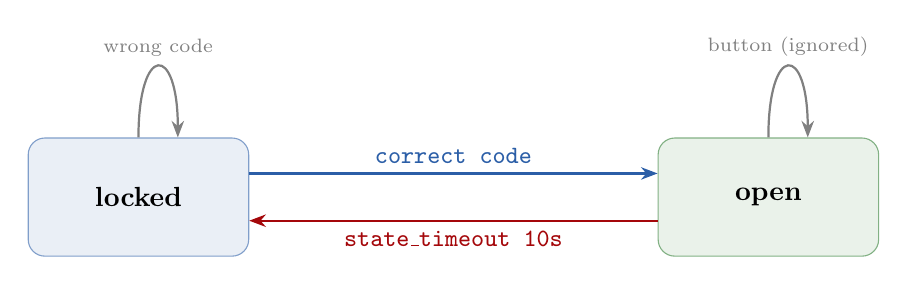
\begin{tikzpicture}[
    state/.style={draw, rounded corners=6pt, fill=#1!10, draw=#1!60,
                  minimum width=2.8cm, minimum height=1.5cm, font=\bfseries},
    trans/.style={-{Stealth[length=6pt]}, thick, #1},
]
    \node[state=erlblue] (locked) at (0, 0) {locked};
    \node[state=erlgreen] (open) at (8, 0) {open};

    % Transitions
    \draw[trans=erlblue] ([yshift=3mm]locked.east) -- node[above, font=\small\ttfamily] {correct code} ([yshift=3mm]open.west);
    \draw[trans=erlred] ([yshift=-3mm]open.west) -- node[below, font=\small\ttfamily] {state\_timeout 10s} ([yshift=-3mm]locked.east);

    % Self-loops
    \draw[trans=gray] (locked.north) .. controls ++(0,1.2) and ++(0,1.2) .. node[above, font=\scriptsize] {wrong code} ([xshift=5mm]locked.north);
    \draw[trans=gray] (open.north) .. controls ++(0,1.2) and ++(0,1.2) .. node[above, font=\scriptsize] {button (ignored)} ([xshift=5mm]open.north);
\end{tikzpicture}
\caption{code\_lock\_state 状态转换图}
\end{figure}

\subsection{模块结构}

\begin{itemize}[leftmargin=2em]
    \item \textbf{模块声明}：\texttt{-behaviour(gen\_statem).} 声明行为模式
    \item \textbf{callback\_mode/0}：返回 \texttt{state\_functions}
    \item \textbf{init/1}：初始化 Data（Map），设置初始状态为 \texttt{locked}
    \item \textbf{locked/3}：处理 \texttt{locked} 状态下的事件（按钮输入）
    \item \textbf{open/3}：处理 \texttt{open} 状态下的事件（超时、按钮）
    \item \textbf{terminate/3}：状态机终止时的清理工作
\end{itemize}

\subsection{使用方式}

\begin{lstlisting}[style=erlangstyle]
%% 1. Start the state machine
{ok, Pid} = code_lock_state:start_link([a, b, c]).

%% 2. Send button events (cast - async)
code_lock_state:button(a).   %% Still locked
code_lock_state:button(b).   %% Still locked
code_lock_state:button(c).   %% Correct code! -> open

%% 3. After 10 seconds, auto-locks via state_timeout
\end{lstlisting}


% ============================================================
% Section 6: All State Events
% ============================================================
\section{公共事件处理 (All State Events)}

\begin{notebox}[源码文件]
\texttt{src/code\_lock\_common.erl}
\end{notebox}

\subsection{问题：多个状态共享相同的事件处理}

某些事件（如查询操作）在所有状态下都需要处理。如果每个状态函数都重复相同的代码，会导致冗余。

\subsection{解决方案：公共处理函数}

在 \texttt{state\_functions} 模式下，使用公共处理函数：

\begin{lstlisting}[style=erlangstyle]
locked(EventType, EventContent, Data) ->
    handle_common(EventType, EventContent, Data).

open(EventType, EventContent, Data) ->
    handle_common(EventType, EventContent, Data).

handle_common({call, From}, code_length, #{code := Code} = Data) ->
    {keep_state, Data, [{reply, From, length(Code)}]}.
\end{lstlisting}

\begin{tipbox}[关键点]
\texttt{code\_length/0} 调用在 \texttt{locked} 和 \texttt{open} 状态下都能工作，因为两个状态函数都委托给了 \texttt{handle\_common/3}。
\end{tipbox}


% ============================================================
% Section 7: Timeout Types
% ============================================================
\section{超时机制}

gen\_statem 提供了四种超时机制，各有不同的取消条件和适用场景。

\subsection{Event Timeout}

\begin{notebox}[源码文件]
\texttt{src/code\_lock\_event\_timeout.erl}
\end{notebox}

\textbf{任何事件到达都会取消}定时器。适用于"如果一段时间内没有任何事件，则执行某操作"。

\begin{lstlisting}[style=erlangstyle]
%% Set event timeout (20 seconds to clear buttons)
{next_state, locked, Data#{buttons := NewButtons}, 20000}
%% Or equivalently:
{next_state, locked, Data, [{timeout, 20000, clear_buttons}]}

%% Handle timeout
locked(timeout, _, Data) ->
    {next_state, locked, Data#{buttons := []}}.
\end{lstlisting}

\subsection{State Timeout}

在\textbf{状态变化时自动取消}。每个状态只能有一个 state\_timeout。适用于"进入某状态后，如果超时则转换状态"。

\begin{lstlisting}[style=erlangstyle]
%% Set state timeout when entering open state
{next_state, open, Data#{buttons := []},
 [{state_timeout, 10000, lock}]}.

%% Handle state timeout
open(state_timeout, lock, Data) ->
    do_lock(),
    {next_state, locked, Data}.
\end{lstlisting}

\subsection{Generic Timeout}

\begin{notebox}[源码文件]
\texttt{src/code\_lock\_generic\_timeout.erl}
\end{notebox}

命名超时，\textbf{不会被事件或状态变化自动取消}。可以有多个不同名称的 generic timeout 同时运行。

\begin{lstlisting}[style=erlangstyle]
%% Set generic timeout with name 'open'
{next_state, open, Data#{buttons := []},
 [{{timeout, open}, 10000, lock}]}.

%% Handle generic timeout
open({timeout, open}, lock, Data) ->
    do_lock(),
    {next_state, locked, Data}.
\end{lstlisting}

\subsection{Erlang Timer}

\begin{notebox}[源码文件]
\texttt{src/code\_lock\_erlang\_timer.erl}
\end{notebox}

使用 \texttt{erlang:start\_timer/3} 创建的定时器，超时消息作为 \texttt{info} 事件到达。最灵活的方式。

\begin{lstlisting}[style=erlangstyle]
%% Start timer
Tref = erlang:start_timer(10000, self(), lock),
{next_state, open, Data#{buttons := [], timer => Tref}}.

%% Handle timer message (arrives as info event)
open(info, {timeout, Tref, lock}, #{timer := Tref} = Data) ->
    do_lock(),
    {next_state, locked, maps:remove(timer, Data)}.
\end{lstlisting}

\subsection{超时类型对比}

\begin{table}[H]
\centering
\begin{tabular}{@{}llll@{}}
\toprule
\textbf{超时类型} & \textbf{设置方式} & \textbf{取消条件} & \textbf{事件类型} \\
\midrule
Event timeout   & \texttt{\{timeout, T, Msg\}} 或 \texttt{T} & 任何事件到达 & \texttt{timeout} \\
State timeout   & \texttt{\{state\_timeout, T, Msg\}} & 状态变化 & \texttt{state\_timeout} \\
Generic timeout & \texttt{\{\{timeout,Name\}, T, Msg\}} & 显式取消/更新 & \texttt{\{timeout,Name\}} \\
Erlang timer    & \texttt{erlang:start\_timer/3} & \texttt{erlang:cancel\_timer/1} & \texttt{info} \\
\bottomrule
\end{tabular}
\caption{四种超时类型对比}
\end{table}


% ============================================================
% Section 8: Postpone
% ============================================================
\section{延迟事件 (Postpone)}

\begin{notebox}[源码文件]
\texttt{src/code\_lock\_postpone.erl}
\end{notebox}

\subsection{概念}

\texttt{postpone} 将当前事件推迟到下一次\textbf{状态变化}后重新处理：

\begin{itemize}[leftmargin=2em]
    \item 事件被放回队列头部
    \item 只有状态变化时，postponed 事件才会被重新投递
    \item 适用于"当前状态无法处理，但换个状态就能处理"
\end{itemize}

\subsection{使用方式}

\begin{lstlisting}[style=erlangstyle]
%% In open state, postpone button events until locked
open(cast, {button, _}, Data) ->
    {keep_state, Data, [postpone]}.
\end{lstlisting}

\subsection{效果}

\begin{figure}[H]
\centering
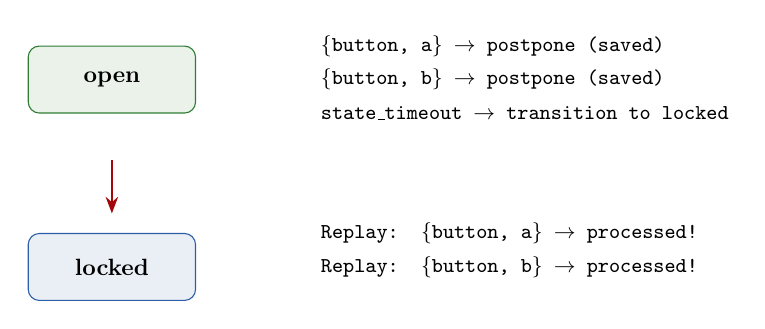
\begin{tikzpicture}[scale=0.85, every node/.style={scale=0.85}]
    % Open state
    \node[draw=erlgreen, fill=erlgreen!10, rounded corners=4pt, minimum width=2.5cm, minimum height=1cm, font=\bfseries] (open) at (0, 0) {open};
    \node[font=\small\ttfamily, anchor=west] at (3, 0.5) {\{button, a\} $\rightarrow$ postpone (saved)};
    \node[font=\small\ttfamily, anchor=west] at (3, 0) {\{button, b\} $\rightarrow$ postpone (saved)};
    \node[font=\small\ttfamily, anchor=west] at (3, -0.5) {state\_timeout $\rightarrow$ transition to locked};

    % Arrow
    \draw[-{Stealth[length=6pt]}, thick, erlred] (0, -1.2) -- (0, -2);

    % Locked state
    \node[draw=erlblue, fill=erlblue!10, rounded corners=4pt, minimum width=2.5cm, minimum height=1cm, font=\bfseries] (locked) at (0, -2.8) {locked};
    \node[font=\small\ttfamily, anchor=west] at (3, -2.3) {Replay: \{button, a\} $\rightarrow$ processed!};
    \node[font=\small\ttfamily, anchor=west] at (3, -2.8) {Replay: \{button, b\} $\rightarrow$ processed!};
\end{tikzpicture}
\caption{postpone 的效果：事件在状态变化后被重新投递}
\end{figure}

\begin{warnbox}[陷阱：postpone 导致无限循环]
如果 postpone 的事件永远不会被处理（状态永远不变），会导致无限循环：
\begin{lstlisting}[style=erlangstyle]
%% BAD: postpone without state change = infinite loop
locked(cast, {button, _}, Data) ->
    {keep_state, Data, [postpone]}.  %% DANGER!
\end{lstlisting}
\end{warnbox}


% ============================================================
% Section 9: State Enter
% ============================================================
\section{状态进入动作 (State Enter)}

\begin{notebox}[源码文件]
\texttt{src/code\_lock\_enter.erl}
\end{notebox}

\subsection{概念}

启用 \texttt{state\_enter} 后，每次状态变化时，gen\_statem 会调用状态回调，事件类型为 \texttt{(enter, OldState, ...)}：

\begin{lstlisting}[style=erlangstyle]
callback_mode() ->
    [state_functions, state_enter].
\end{lstlisting}

\subsection{使用方式}

\begin{lstlisting}[style=erlangstyle]
%% Enter action: lock the door and clear buttons
locked(enter, _OldState, Data) ->
    do_lock(),
    {keep_state, Data#{buttons => []}};

locked(cast, {button, Button}, Data) ->
    ...

%% Enter action: unlock the door and set state timeout
open(enter, _OldState, _Data) ->
    do_unlock(),
    {keep_state_and_data, [{state_timeout, 10000, lock}]};

open(state_timeout, lock, Data) ->
    {next_state, locked, Data}.
\end{lstlisting}

\subsection{优势}

\begin{itemize}[leftmargin=2em]
    \item 将状态初始化逻辑集中在 enter 处理中
    \item \texttt{init/1} 不需要手动调用 \texttt{do\_lock()}
    \item 可以用 \texttt{repeat\_state} 重新触发 enter 动作
\end{itemize}

\begin{warnbox}[注意]
在 enter 处理中，\textbf{必须}返回 \texttt{keep\_state} 系列，不能返回 \texttt{next\_state}：
\begin{lstlisting}[style=erlangstyle]
%% BAD: state enter must not change state
locked(enter, _OldState, Data) ->
    {next_state, open, Data}.  %% CRASH!

%% GOOD: use keep_state in enter
locked(enter, _OldState, Data) ->
    {keep_state, Data#{buttons => []}}.
\end{lstlisting}
\end{warnbox}


% ============================================================
% Section 10: Inserted Events
% ============================================================
\section{插入事件 (Inserted Events)}

\begin{notebox}[源码文件]
\texttt{src/code\_lock\_inserted.erl}
\end{notebox}

\subsection{概念}

使用 \texttt{\{next\_event, EventType, EventContent\}} 动作可以在当前状态插入新事件：

\begin{itemize}[leftmargin=2em]
    \item 插入的事件在下一个事件之前被处理
    \item 常用于将外部事件转换为内部事件
    \item \texttt{internal} 事件类型只能通过 \texttt{next\_event} 产生
\end{itemize}

\subsection{使用方式：按键的 down/up 事件}

\begin{lstlisting}[style=erlangstyle]
%% Convert up event to internal button event
handle_common(cast, {up, Button}, Data) ->
    case Data of
        #{button := Button} ->
            {keep_state, maps:remove(button, Data),
             [{next_event, internal, {button, Button}}]};
        #{} ->
            keep_state_and_data
    end.

%% Handle the internal event
locked(internal, {button, Button}, Data) ->
    %% Process button press...
\end{lstlisting}


% ============================================================
% Section 11: Complex State
% ============================================================
\section{复杂状态 (Complex State)}

\begin{notebox}[源码文件]
\texttt{src/code\_lock\_complex.erl}
\end{notebox}

\subsection{概念}

在 \texttt{handle\_event\_function} 模式下，状态可以是任意 term，不限于 atom。例如使用元组 \texttt{\{StateName, LockButton\}} 作为状态：

\begin{lstlisting}[style=erlangstyle]
init({Code, LockButton}) ->
    Data = #{code => Code, length => length(Code), buttons => []},
    {ok, {locked, LockButton}, Data}.

callback_mode() ->
    [handle_event_function, state_enter].

%% State: {locked, LockButton}
handle_event(enter, _OldState, {locked, _}, Data) ->
    do_lock(),
    {keep_state, Data#{buttons := []}};

%% State: {open, LockButton}
handle_event(cast, {button, LockButton}, {open, LockButton}, Data) ->
    {next_state, {locked, LockButton}, Data};

%% Common: change lock button in any state
handle_event({call, From}, {set_lock_button, NewLB},
             {StateName, OldLB}, Data) ->
    {next_state, {StateName, NewLB}, Data,
     [{reply, From, OldLB}]}.
\end{lstlisting}

\begin{tipbox}[复杂状态的优势]
\begin{itemize}[leftmargin=1.5em]
    \item 状态可以携带额外信息（如 \texttt{LockButton}）
    \item 利用模式匹配精确路由事件
    \item 运行时可以动态修改状态的组成部分
    \item 适合需要参数化状态的场景
\end{itemize}
\end{tipbox}


% ============================================================
% Section 12: Stopping
% ============================================================
\section{停止 gen\_statem}

\begin{notebox}[源码文件]
\texttt{src/code\_lock\_stop.erl}
\end{notebox}

\subsection{在监督树中}

在监督树中，gen\_statem 通过 supervisor 的关闭策略停止。需要在 \texttt{init/1} 中设置 \texttt{process\_flag(trap\_exit, true)}。

\subsection{独立停止}

\begin{lstlisting}[style=erlangstyle]
%% API function
stop() ->
    gen_statem:stop(code_lock).

%% Or with reason and timeout
gen_statem:stop(code_lock, normal, 5000).
\end{lstlisting}

\subsection{terminate/3 回调}

\begin{lstlisting}[style=erlangstyle]
terminate(Reason, State, Data) ->
    %% Cleanup resources
    State =/= locked andalso do_lock(),
    ok.
\end{lstlisting}

\begin{warnbox}[注意]
\texttt{terminate/3} 只在以下情况被调用：
\begin{itemize}
    \item 回调函数返回 \texttt{\{stop, ...\}}
    \item 进程收到 EXIT 信号且设置了 \texttt{process\_flag(trap\_exit, true)}
    \item \texttt{gen\_statem:stop/1,3} 被调用
\end{itemize}
\end{warnbox}


% ============================================================
% Section 13: Callback Return Values
% ============================================================
\section{回调函数返回值}

\subsection{init/1}

\begin{lstlisting}[style=erlangstyle]
init(Args) ->
    {ok, State, Data}                %% Normal start
  | {ok, State, Data, Actions}       %% Start with actions
  | {stop, Reason}                   %% Start failed
  | ignore.                          %% Ignore start
\end{lstlisting}

\subsection{状态回调返回值}

\begin{lstlisting}[style=erlangstyle]
%% State transition
{next_state, NextState, NewData}
{next_state, NextState, NewData, Actions}

%% Stay in current state
{keep_state, NewData}
{keep_state, NewData, Actions}
keep_state_and_data
{keep_state_and_data, Actions}

%% Repeat state enter (only with state_enter)
{repeat_state, NewData}
{repeat_state, NewData, Actions}
repeat_state_and_data
{repeat_state_and_data, Actions}

%% Stop
{stop, Reason}
{stop, Reason, NewData}
{stop_and_reply, Reason, Replies}
{stop_and_reply, Reason, Replies, NewData}
\end{lstlisting}

\subsection{Actions (动作)}

\begin{lstlisting}[style=erlangstyle]
Actions = [Action]
Action =
    postpone                                    %% Postpone current event
  | {postpone, boolean()}
  | {next_event, EventType, EventContent}       %% Insert event
  | {reply, From, Reply}                        %% Reply to call
  | {state_timeout, Time, EventContent}         %% State timeout
  | {state_timeout, update, EventContent}       %% Update state timeout
  | {state_timeout, cancel}                     %% Cancel state timeout
  | {{timeout, Name}, Time, EventContent}       %% Generic timeout
  | {{timeout, Name}, update, EventContent}     %% Update generic timeout
  | {{timeout, Name}, cancel}                   %% Cancel generic timeout
  | {timeout, Time, EventContent}               %% Event timeout
  | Time                                        %% Event timeout (integer)
  | hibernate.                                  %% Hibernate process
\end{lstlisting}


% ============================================================
% Section 14: Message Flow
% ============================================================
\section{消息流转}

\begin{figure}[H]
\centering
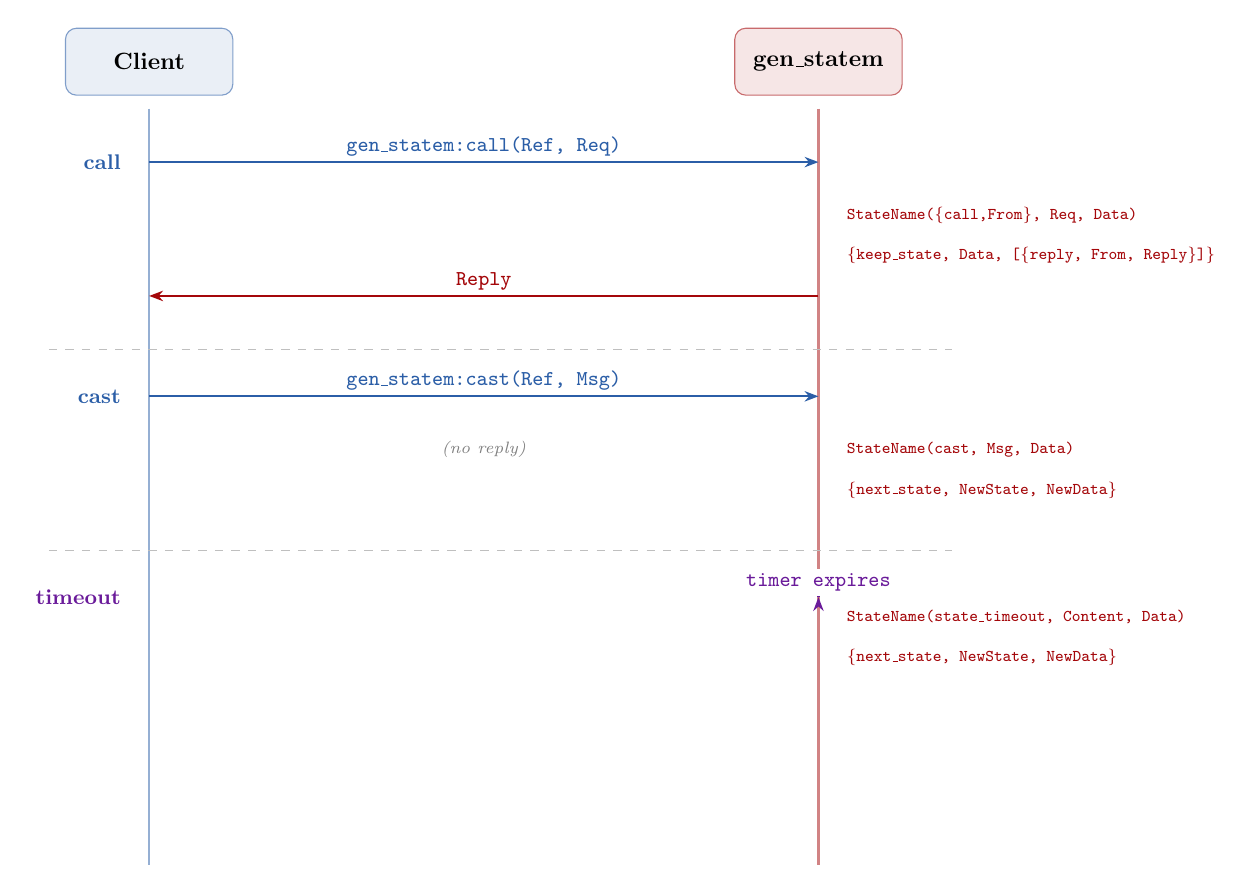
\begin{tikzpicture}[scale=0.85, every node/.style={scale=0.85},
    actor/.style={draw, rounded corners=4pt, fill=#1!10, draw=#1!60,
                  minimum width=2.5cm, minimum height=1cm, font=\bfseries},
    msg/.style={-{Stealth[length=5pt]}, thick, #1},
    lbl/.style={font=\small\ttfamily, fill=white, inner sep=2pt},
]
    \node[actor=erlblue] (client) at (0, 0) {Client};
    \node[actor=erlred] (server) at (10, 0) {gen\_statem};

    \draw[thick, erlblue!50] (0, -0.7) -- (0, -12);
    \draw[thick, erlred!50] (10, -0.7) -- (10, -12);

    % === call ===
    \node[font=\small\bfseries\color{erlblue}, anchor=east] at (-0.3, -1.5) {call};
    \draw[msg=erlblue] (0, -1.5) -- node[lbl, above] {gen\_statem:call(Ref, Req)} (10, -1.5);
    \node[font=\scriptsize\ttfamily, anchor=west, text=erlred] at (10.3, -2.3) {StateName(\{call,From\}, Req, Data)};
    \node[font=\scriptsize\ttfamily, anchor=west, text=erlred] at (10.3, -2.9) {\{keep\_state, Data, [\{reply, From, Reply\}]\}};
    \draw[msg=erlred] (10, -3.5) -- node[lbl, above] {Reply} (0, -3.5);

    % === cast ===
    \node[font=\small\bfseries\color{erlblue}, anchor=east] at (-0.3, -5) {cast};
    \draw[msg=erlblue] (0, -5) -- node[lbl, above] {gen\_statem:cast(Ref, Msg)} (10, -5);
    \node[font=\scriptsize\ttfamily, anchor=west, text=erlred] at (10.3, -5.8) {StateName(cast, Msg, Data)};
    \node[font=\scriptsize\ttfamily, anchor=west, text=erlred] at (10.3, -6.4) {\{next\_state, NewState, NewData\}};
    \node[font=\scriptsize\itshape\color{gray}] at (5, -5.8) {(no reply)};

    % === timeout ===
    \node[font=\small\bfseries\color{erlpurple}, anchor=east] at (-0.3, -8) {timeout};
    \node[font=\scriptsize\ttfamily, anchor=west, text=erlred] at (10.3, -8.3) {StateName(state\_timeout, Content, Data)};
    \node[font=\scriptsize\ttfamily, anchor=west, text=erlred] at (10.3, -8.9) {\{next\_state, NewState, NewData\}};
    \draw[msg=erlpurple, dashed] (10, -8) -- node[lbl, above] {timer expires} (10, -8);

    % Dashed separators
    \draw[dashed, gray!50] (-1.5, -4.3) -- (12, -4.3);
    \draw[dashed, gray!50] (-1.5, -7.3) -- (12, -7.3);
\end{tikzpicture}
\caption{gen\_statem 消息流转过程}
\label{fig:message-flow}
\end{figure}

\subsection{状态转换流程}

\begin{figure}[H]
\centering
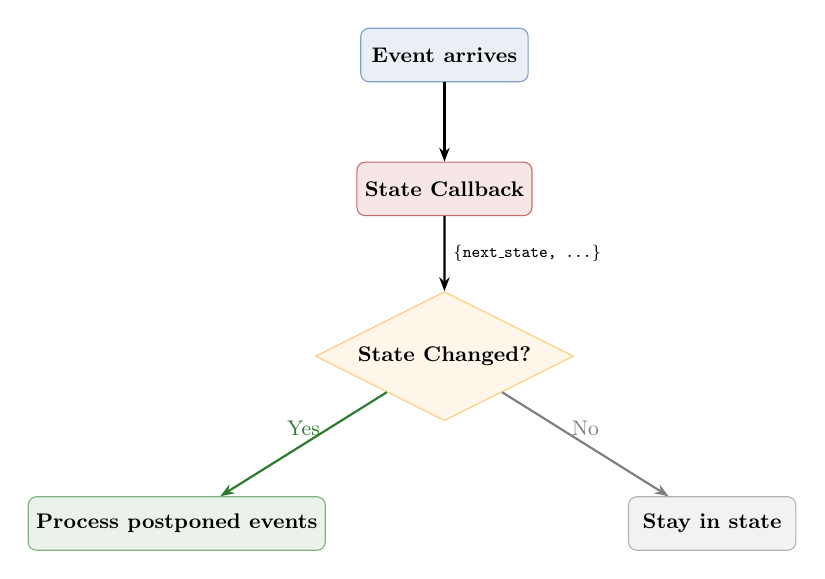
\begin{tikzpicture}[scale=0.85, every node/.style={scale=0.85},
    box/.style={draw, rounded corners=3pt, fill=#1!10, draw=#1!60,
                minimum width=2.5cm, minimum height=0.8cm, font=\small\bfseries},
    decision/.style={draw, diamond, fill=erlyellow!10, draw=erlyellow!60,
                     minimum width=2cm, minimum height=1cm, font=\small\bfseries,
                     aspect=2},
]
    \node[box=erlblue] (event) at (0, 0) {Event arrives};
    \node[box=erlred] (callback) at (0, -2) {State Callback};
    \node[decision] (changed) at (0, -4.5) {State Changed?};
    \node[box=erlgreen] (replay) at (-4, -7) {Process postponed events};
    \node[box=gray] (stay) at (4, -7) {Stay in state};

    \draw[-{Stealth[length=5pt]}, thick] (event) -- (callback);
    \draw[-{Stealth[length=5pt]}, thick] (callback) -- node[right, font=\scriptsize\ttfamily] {\{next\_state, ...\}} (changed);
    \draw[-{Stealth[length=5pt]}, thick, erlgreen] (changed) -- node[above, font=\small] {Yes} (replay);
    \draw[-{Stealth[length=5pt]}, thick, gray] (changed) -- node[above, font=\small] {No} (stay);
\end{tikzpicture}
\caption{状态转换流程}
\end{figure}


% ============================================================
% Section 15: Best Practices
% ============================================================
\section{最佳实践与常见陷阱}

\subsection{最佳实践}

\begin{enumerate}[leftmargin=2em]
    \item \textbf{优先使用 state\_functions}：代码更清晰，每个状态一个函数
    \item \textbf{使用 state\_enter}：将状态初始化逻辑集中管理
    \item \textbf{善用 postpone}：避免在错误状态下丢弃事件
    \item \textbf{使用 state\_timeout}：比 event timeout 更可预测
    \item \textbf{trap\_exit}：在监督树中使用时设置 \texttt{process\_flag(trap\_exit, true)}
    \item \textbf{处理所有状态的公共事件}：使用 \texttt{handle\_common} 避免代码重复
\end{enumerate}

\subsection{常见陷阱}

\subsubsection{陷阱 1：忘记处理所有状态的公共事件}

\begin{lstlisting}[style=erlangstyle]
%% BAD: code_length only works in locked state
locked({call, From}, code_length, Data) ->
    {keep_state, Data, [{reply, From, length(maps:get(code, Data))}]}.
%% open state will crash on code_length call!

%% GOOD: handle in all states
locked(EventType, EventContent, Data) ->
    handle_common(EventType, EventContent, Data).
open(EventType, EventContent, Data) ->
    handle_common(EventType, EventContent, Data).
\end{lstlisting}

\subsubsection{陷阱 2：postpone 导致无限循环}

\begin{lstlisting}[style=erlangstyle]
%% BAD: postpone without state change = infinite loop
locked(cast, {button, _}, Data) ->
    {keep_state, Data, [postpone]}.  %% DANGER! Never changes state
\end{lstlisting}

\subsubsection{陷阱 3：混淆超时类型}

\begin{lstlisting}[style=erlangstyle]
%% event timeout: cancelled by ANY event
{next_state, State, Data, [{timeout, 5000, msg}]}

%% state timeout: cancelled by state CHANGE
{next_state, State, Data, [{state_timeout, 5000, msg}]}

%% generic timeout: only cancelled explicitly
{next_state, State, Data, [{{timeout, name}, 5000, msg}]}
\end{lstlisting}

\subsubsection{陷阱 4：state\_enter 中返回 next\_state}

\begin{lstlisting}[style=erlangstyle]
%% BAD: state enter must not change state
locked(enter, _OldState, Data) ->
    {next_state, open, Data}.  %% CRASH!

%% GOOD: use keep_state in enter
locked(enter, _OldState, Data) ->
    {keep_state, Data#{buttons => []}}.
\end{lstlisting}


% ============================================================
% Section 16: Quick Reference
% ============================================================
\section{快速参考}

\subsection{启动函数}

\begin{table}[H]
\centering
\begin{tabular}{@{}ll@{}}
\toprule
\textbf{函数} & \textbf{说明} \\
\midrule
\texttt{gen\_statem:start\_link(\{local,N\}, Mod, Args, Opts)} & 启动并本地注册 \\
\texttt{gen\_statem:start\_link(\{global,N\}, Mod, Args, Opts)} & 启动并全局注册 \\
\texttt{gen\_statem:start\_link(Mod, Args, Opts)} & 启动不注册 \\
\texttt{gen\_statem:start(...)} & 同上但不链接 \\
\texttt{gen\_statem:stop(Ref)} & 停止状态机 \\
\bottomrule
\end{tabular}
\caption{启动函数}
\end{table}

\subsection{消息发送函数}

\begin{table}[H]
\centering
\begin{tabular}{@{}lll@{}}
\toprule
\textbf{函数} & \textbf{类型} & \textbf{说明} \\
\midrule
\texttt{gen\_statem:call(Ref, Req)} & 同步 & 发送请求并等待回复 \\
\texttt{gen\_statem:call(Ref, Req, Timeout)} & 同步 & 带超时 \\
\texttt{gen\_statem:cast(Ref, Msg)} & 异步 & 发送异步消息 \\
\texttt{Ref ! Msg} & 异步 & 发送 info 消息 \\
\bottomrule
\end{tabular}
\caption{消息发送函数}
\end{table}

\subsection{回调函数}

\begin{lstlisting}[style=erlangstyle]
init/1:
  {ok, State, Data}
  {ok, State, Data, Actions}
  {stop, Reason}
  ignore

callback_mode/0:
  state_functions | handle_event_function
  | [CallbackMode]
  | [CallbackMode, state_enter]

StateName/3 (state_functions mode):
  StateName(EventType, EventContent, Data) -> Result

handle_event/4 (handle_event_function mode):
  handle_event(EventType, EventContent, State, Data) -> Result

terminate/3:
  terminate(Reason, State, Data) -> Ignored

code_change/4:
  code_change(OldVsn, State, Data, Extra) -> {ok, NewState, NewData}
\end{lstlisting}

\subsection{源码文件列表}

\begin{table}[H]
\centering
\begin{tabular}{@{}lll@{}}
\toprule
\textbf{文件} & \textbf{说明} & \textbf{对应章节} \\
\midrule
\texttt{src/code\_lock\_state.erl} & 基本用法：state\_functions 模式 & \S5 \\
\texttt{src/code\_lock\_handle\_event.erl} & handle\_event\_function 模式 & \S4 \\
\texttt{src/code\_lock\_common.erl} & All State Events (公共事件) & \S6 \\
\texttt{src/code\_lock\_stop.erl} & 停止 gen\_statem & \S12 \\
\texttt{src/code\_lock\_event\_timeout.erl} & Event Time-Outs & \S7 \\
\texttt{src/code\_lock\_generic\_timeout.erl} & Generic Time-Outs & \S7 \\
\texttt{src/code\_lock\_erlang\_timer.erl} & Erlang Timers & \S7 \\
\texttt{src/code\_lock\_postpone.erl} & Postponing Events & \S8 \\
\texttt{src/code\_lock\_enter.erl} & State Enter Actions & \S9 \\
\texttt{src/code\_lock\_inserted.erl} & Inserted Events (down/up) & \S10 \\
\texttt{src/code\_lock\_complex.erl} & Complex State & \S11 \\
\texttt{src/code\_lock\_selective.erl} & Selective Receive (原生实现) & --- \\
\texttt{src/lock\_state\_pid.erl} & server\_ref 演示：PID 方式 & \S2 \\
\texttt{src/lock\_state\_local.erl} & server\_ref 演示：本地注册 & \S3 \\
\texttt{src/lock\_state\_global.erl} & server\_ref 演示：全局注册 & \S3 \\
\bottomrule
\end{tabular}
\caption{源码文件列表}
\end{table}

\subsection{Makefile 命令}

\begin{lstlisting}[style=shellstyle, caption={src/Makefile 可用命令}]
make compile            # Compile all .erl files
make run_state          # Basic state_functions demo
make run_handle_event   # handle_event_function demo
make run_common         # All State Events demo
make run_stop           # Stop demo
make run_event_timeout  # Event timeout demo
make run_generic_timeout # Generic timeout demo
make run_erlang_timer   # Erlang timer demo
make run_postpone       # Postpone demo
make run_enter          # State enter demo
make run_inserted       # Inserted events (down/up) demo
make run_complex        # Complex state demo
make run_selective      # Selective receive demo
make run_all            # Run all demos sequentially
make clean              # Remove compiled files
\end{lstlisting}


\end{document}
